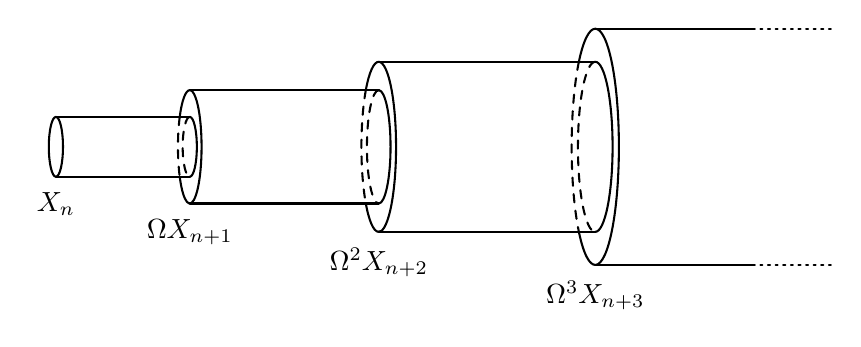
\begin{tikzpicture}[x=1cm,y=1cm,line width=.75pt,
                    line cap=round,line join=round]
  % Tapa izquierda completamente visible.
  \def\tapaVisible#1#2#3{%
    \draw (#1,0) ellipse [x radius=#2,y radius=#3];%
  }

  % Tapa derecha: mitad izquierda oculta.
  \def\tapaDerecha#1#2#3{%
    \draw[dashed] (#1,#3)
      arc[start angle=90,end angle=270,
          x radius=#2,y radius=#3];
    \draw (#1,#3)
      arc[start angle=90,end angle=-90,
          x radius=#2,y radius=#3];%
  }

  % Tapa izquierda: arco oculto por el cilindro anterior.
  \def\tapaIzquierda#1#2#3#4{%
    \pgfmathsetmacro{\anguloOculto}{asin(#4/#3)}%
    \draw (#1,#3)
      arc[start angle=90,end angle={180-\anguloOculto},
          x radius=#2,y radius=#3];
    \draw[dashed] ({#1-#2*cos(\anguloOculto)},#4)
      arc[start angle={180-\anguloOculto},
          end angle={180+\anguloOculto},
          x radius=#2,y radius=#3];
    \draw ({#1-#2*cos(\anguloOculto)},{-#4})
      arc[start angle={180+\anguloOculto},end angle=450,
          x radius=#2,y radius=#3];%
  }

  % Primer cilindro.
  \draw (2.55,.38) -- (4.25,.38)
        (2.55,-.38) -- (4.25,-.38);
  \tapaVisible{2.55}{.09}{.38}
  \tapaDerecha{4.25}{.09}{.38}
  \node[below=2pt] at (2.55,-.38) {$X_n$};

  % Segundo cilindro.
  \draw (4.25,.72) -- (6.65,.72)
        (4.25,-.72) -- (6.65,-.72);
  \tapaIzquierda{4.25}{.15}{.72}{.38}
  \tapaDerecha{6.65}{.15}{.72}
  \node[below=2pt] at (4.25,-.72) {$\Omega X_{n+1}$};

  % Tercer cilindro.
  \draw (6.65,1.08) -- (9.40,1.08)
        (6.65,-1.08) -- (9.40,-1.08);
  \tapaIzquierda{6.65}{.22}{1.08}{.72}
  \tapaDerecha{9.40}{.22}{1.08}
  \node[below=2pt] at (6.65,-1.08) {$\Omega^2 X_{n+2}$};

  % Último cilindro: continuación indefinida, sin tapa derecha.
  \tapaIzquierda{9.40}{.30}{1.50}{1.08}
  \draw (9.40,1.50) -- (11.40,1.50)
        (9.40,-1.50) -- (11.40,-1.50);
  \draw[dotted] (11.40,1.50) -- (12.40,1.50)
                (11.40,-1.50) -- (12.40,-1.50);
  \node[below=2pt] at (9.40,-1.50) {$\Omega^3 X_{n+3}$};
\end{tikzpicture}